\documentclass[a4paper, 11pt]{report}\usepackage[]{graphicx}\usepackage[]{color}
%% maxwidth is the original width if it is less than linewidth
%% otherwise use linewidth (to make sure the graphics do not exceed the margin)
\makeatletter
\def\maxwidth{ %
  \ifdim\Gin@nat@width>\linewidth
    \linewidth
  \else
    \Gin@nat@width
  \fi
}
\makeatother

\definecolor{fgcolor}{rgb}{0.345, 0.345, 0.345}
\newcommand{\hlnum}[1]{\textcolor[rgb]{0.686,0.059,0.569}{#1}}%
\newcommand{\hlstr}[1]{\textcolor[rgb]{0.192,0.494,0.8}{#1}}%
\newcommand{\hlcom}[1]{\textcolor[rgb]{0.678,0.584,0.686}{\textit{#1}}}%
\newcommand{\hlopt}[1]{\textcolor[rgb]{0,0,0}{#1}}%
\newcommand{\hlstd}[1]{\textcolor[rgb]{0.345,0.345,0.345}{#1}}%
\newcommand{\hlkwa}[1]{\textcolor[rgb]{0.161,0.373,0.58}{\textbf{#1}}}%
\newcommand{\hlkwb}[1]{\textcolor[rgb]{0.69,0.353,0.396}{#1}}%
\newcommand{\hlkwc}[1]{\textcolor[rgb]{0.333,0.667,0.333}{#1}}%
\newcommand{\hlkwd}[1]{\textcolor[rgb]{0.737,0.353,0.396}{\textbf{#1}}}%

\usepackage{framed}
\makeatletter
\newenvironment{kframe}{%
 \def\at@end@of@kframe{}%
 \ifinner\ifhmode%
  \def\at@end@of@kframe{\end{minipage}}%
  \begin{minipage}{\columnwidth}%
 \fi\fi%
 \def\FrameCommand##1{\hskip\@totalleftmargin \hskip-\fboxsep
 \colorbox{shadecolor}{##1}\hskip-\fboxsep
     % There is no \\@totalrightmargin, so:
     \hskip-\linewidth \hskip-\@totalleftmargin \hskip\columnwidth}%
 \MakeFramed {\advance\hsize-\width
   \@totalleftmargin\z@ \linewidth\hsize
   \@setminipage}}%
 {\par\unskip\endMakeFramed%
 \at@end@of@kframe}
\makeatother

\definecolor{shadecolor}{rgb}{.97, .97, .97}
\definecolor{messagecolor}{rgb}{0, 0, 0}
\definecolor{warningcolor}{rgb}{1, 0, 1}
\definecolor{errorcolor}{rgb}{1, 0, 0}
\newenvironment{knitrout}{}{} % an empty environment to be redefined in TeX

\usepackage{alltt}
\usepackage[T1]{fontenc}
\usepackage{amsmath}
\usepackage[margin = 1in]{geometry}
\usepackage{mathpazo}
\usepackage[natbib=true, backend=bibtex, style=numeric, citestyle=authoryear]{biblatex}
\usepackage{apalike}
\usepackage{appendix}
\usepackage[margin = 1cm, justification = centering]{caption}
\usepackage[margin = 0.25cm, justification = centering]{subcaption}
\usepackage{pgf, tikz}
\usepackage{setspace}
\usepackage{float}
\usepackage{wrapfig}


\usetikzlibrary{positioning}
\addbibresource{references.bib}
\numberwithin{figure}{section}


\title{\Large{A report on} \\ \vspace{0.5cm}
Heart Rate Variablility (HVR) Signal Analysis \\ \vfill 
\Large{\textsc{Compulsory Assignment} \\ \vspace{1cm}
Multivariate Data and Meta Modeling: Preparing for Big Data Cybernetics} \vfill}
\author{Raju Rimal and Veronika Lindberg}


\onehalfspacing
\IfFileExists{upquote.sty}{\usepackage{upquote}}{}
\begin{document}
\maketitle
\tableofcontents

\chapter{Overview}
The exploration of Heart Rate Variablity signal data is the main objective of this project. Heart Rate of a person vary according to the state of a person whether s(he) is sleeping or resting or engaged in some activities. Samples are collected with startified random sampling from several persons under various conditions to maximize the variablity in the colleced dataset. A soft modelling approach is implemented in the bilinear model in the project. The models were accessed by graphical interpretation and cross-validation. The approach applied in the project is summarized in the figure - ref{fig:projectOverview}, where an inductive exploration of data is made in the initial part and deductive data driven meta-modeling is performed in the final part.

\begin{figure}[H]
\begin{tikzpicture}
  \node (top-left) at (0,0) {
    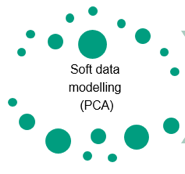
\includegraphics[width = 0.18\textwidth]{figure/overview_fig_1}};
  \node [below = of top-left] (bottom-left) {
    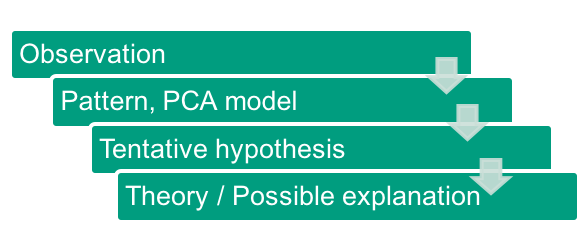
\includegraphics[width = 0.45\textwidth]{figure/overview_fig_3}};
  \node [right = of bottom-left] (bottom-right) {
    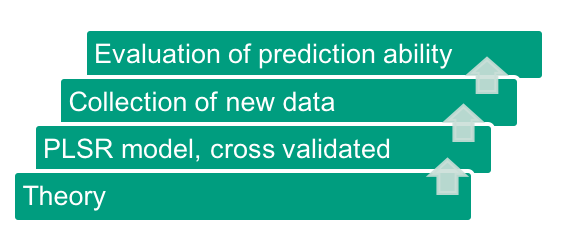
\includegraphics[width = 0.45\textwidth]{figure/overview_fig_4}};
  \node [above = of bottom-right] (top-right) {
    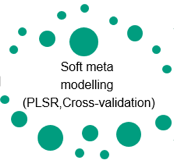
\includegraphics[width = 0.18\textwidth]{figure/overview_fig_2}};
\end{tikzpicture}
\caption{Approach implemented in the Project}
\label{fig:projectOverview}
\end{figure}

\chapter{Heart Rate Variability (HRV)}
Heart Rate Variablility (HRV) is the variation in the time interal between heartbeats. In an ECG plot shown in figure-\ref{fig:ecgSignal}, the interval between heartbeats can be seen as the interval between the dominant R peaks.
\begin{figure}[H]
\centering
\begin{subfigure}[b]{0.49\textwidth}
  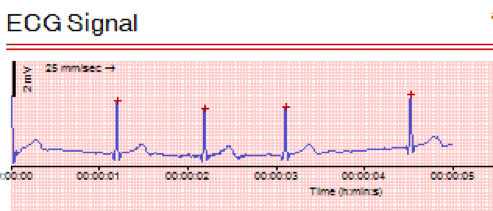
\includegraphics[width = \textwidth]{figure/ecg-1}
  \caption{A general ECG signal}
\end{subfigure}
\begin{subfigure}[b]{0.49\textwidth}
  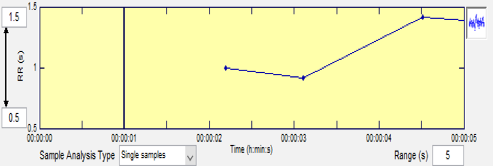
\includegraphics[width = \textwidth]{figure/ecg-2}
  \caption{The RR-interval for ECG signal}
\end{subfigure}
\caption{The four peaks in the ECG signal gives three RR-intervals}
\label{fig:ecgSignal}
\end{figure}

\begin{wrapfigure}{rh}{0.37\textwidth}
\vspace{-10pt}
  \begin{center}
    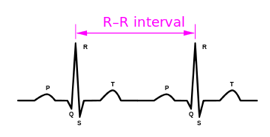
\includegraphics[width=0.35\textwidth]{figure/ecg-3}
  \end{center}
  \caption{A ECG signal model with illustrated RR-interval} 
  \label{fig:modelECG}
  \vspace{-50pt}
\end{wrapfigure}

The peaks are easier to detect and its distance can be measured as RR interval series also known as HRV series. In the figure-\ref{fig:modelECG}, the RR distance is shown by pink double arrow. These distance between the peaks differ and the series itself vary accross different state of a person.
\section{Heart Rate Variability and Body Resilience}
The Autonomic nervous system plays an important role in the regulation of the heart rate.

\begin{itemize}
\item The Sympathetic part, or the ``Fight or Flight response'' contributes to a higher heart rate.
\item The Parasympathetic part, or the “Rest and Repair response” contributes to a lower heart rate.
\item Both parts contributes to the HRV variation.
\end{itemize}

\begin{figure}[H]
\centering
\begin{subfigure}[t]{0.47\textwidth}
  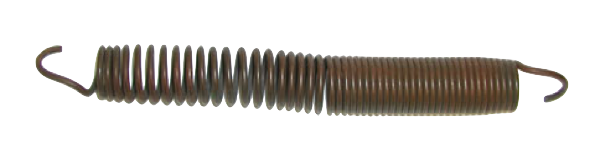
\includegraphics[width = \textwidth]{figure/Spring}
  \caption{An overstretched tension spring has lost some of its elasticity}
\end{subfigure}
\begin{subfigure}[t]{0.47\textwidth}
  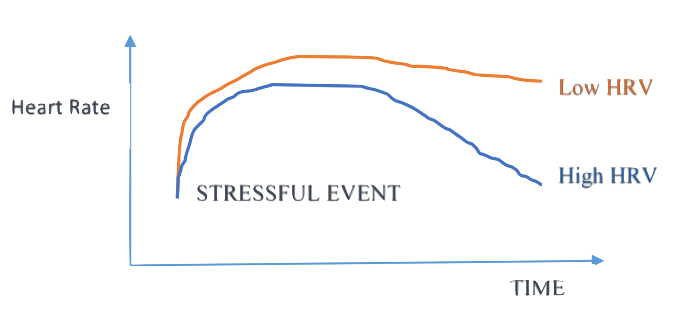
\includegraphics[width = \textwidth]{figure/hvr_low_high}
  \caption{The RR-interval obtained from the ECG signal}
\end{subfigure}
\caption{An person with low HRV has lost some of the ability to calm down after a stressful event}
\label{fig:hrProperties}
\end{figure}

A healthy person with a well functioning autonomic nervous system will typically have a high HRV, and will be able to adapt to changes. However a sick person or a person in poor physical condition, will typically have a low HRV, and will have insufficient ability to adapt to changes.

\section{Application of HR and HRV measurement}
Both Heart Rate and Heart Rate Variability are widely used as non-invasive measurements. The ranges for normal HR and HRV vary by body size, physical condition, body position, time of day and more.
\begin{description}
\item [Sports:] \hfill \\
Athletes need to push themselves hard to perform better, and HR and HRV analysis are used to avoid over training, and in the recovering phase after illness or overexertion. 
\begin{description}
\item [High HRV:] Can do hard exercises
\item [Increasing HRV:] In risk of over training
\item [Low HRV:] Over trained, need rest
\end{description}
\item [Psychology:]\hfill \\ 
Breathing exercises, yoga type exercises, visualization techniques, mindfulness and similar techniques are used together with HR and HRV analysis in stress management. 
\item [Medicine:]\hfill \\ 
HR and HRV analysis give an invasive window to the autonomic nervous system. Decreased in HRV is found to be a strong indicator of impaired health. Physical activity is found to increase HRV in both healthy persons and in patients with diseases. Both inactivity and overexertion reduces the HRV, and increases therefore the risk of diseases.
\item [Traditional Medicine:]\hfill \\ 
\end{description}
Heart Rate and HRV can be measured using instruments like ECG, Optical sensors and Bio impedance sensors. In mordern days, wearable sensors like Chest straps and wristbands are also in use for HRV measurement.

\section{RR intervals as time series}
The RR interval is measured as the interval between consecutive heart beats, measured in seconds or milliseconds (fig-\ref{fig:rrSeries}). The time line is created by adding the consecutive RR intervals. The instantaneous HR is the invers of the RR value. HR is usually measured as an average value of the heart beats over a period of time, as beats per minute (fig-\ref{fig:hrSeries}). The Polar H7 device, used in this project, reports both RR intervals and average HR values. 

\begin{figure}[H]
\centering
\begin{subfigure}[t]{0.47\textwidth}
  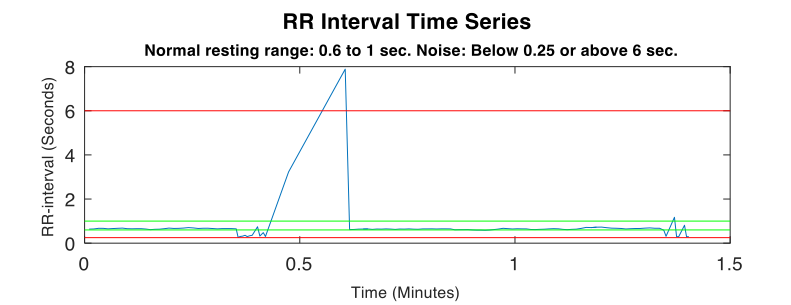
\includegraphics[width = \textwidth]{figure/rrTimeSeriesTop}
  \caption{RR interval Time Series}
  \label{fig:rrSeries}
\end{subfigure}
\begin{subfigure}[t]{0.47\textwidth}
  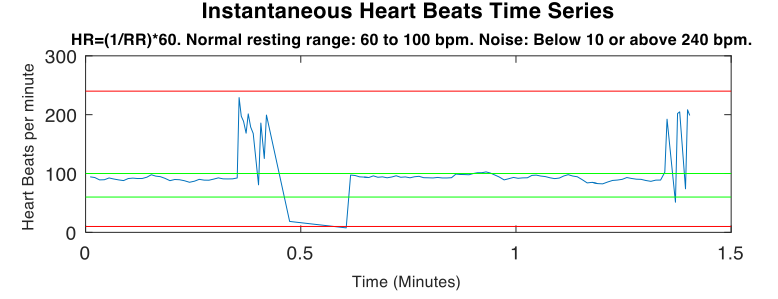
\includegraphics[width = \textwidth]{figure/rrTimeSeriesBottom}
  \caption{Instantaneous Heart Beats Time Series}
  \label{fig:hrSeries}
\end{subfigure}
\caption{RR interval and Heart Beats presented as Time Series}
\label{fig:rr.hrv.timeseries}
\end{figure}

Here, we have used the instantaneous RR intervals in our project. RR intervals shorter than 0.25 msec are not reported by the device – because this is the physical minimum duration of the heart contraction in an adult. RR intervals longer than 2 msec can mean either that the device has lost some beats, or that the heart is not contracting for a while.
HRV analysis can be done with or without artifact correction.

\section{Variation of HRV among persons}
Heart rate variability varies among person to person accordance to their state. Such as, HRV for a young and elder person is different and similarly an ill person and healthly person also have quite differnt HRV series (fig-\ref{fig:hrv.variation}). The HRV series also vary according to the activities of the person.
\begin{figure}[H]
\centering
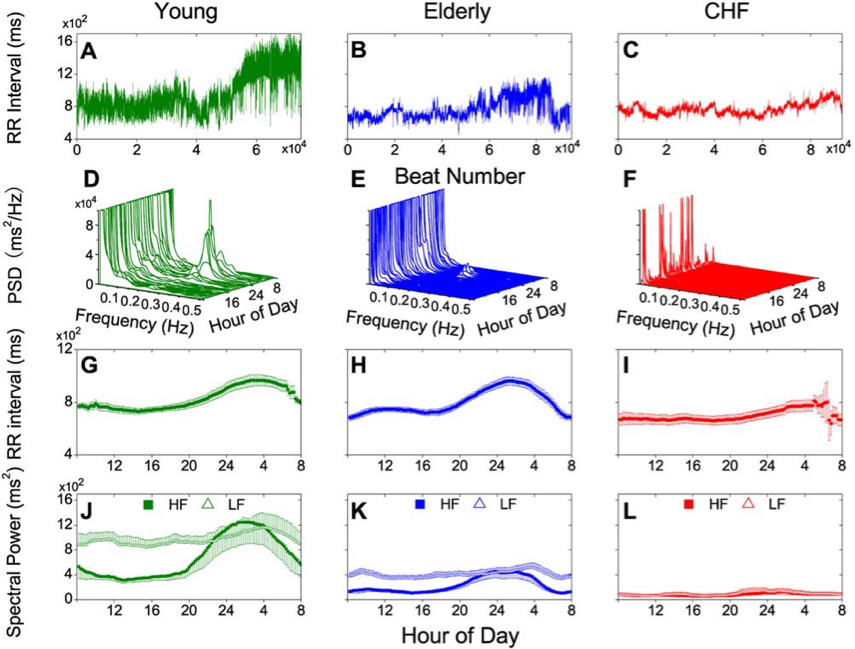
\includegraphics[width = 0.8\textwidth]{figure/hrvVariation}
\caption{HRV variation among young, elder and ill Person}
\label{fig:hrv.variation}
\end{figure}

Young and healthy persons have a greater hearth rate variability than older or ill persons. Some frequencies are present only during sleep. The RR-intervals follow a 24-hour cycle. The ratio between high and low frequencies is a widely used measurement of body resilience. The ratio is usually evaluated in the morning. (Sports: Morning readiness)

\chapter{Data Collection and Preprocessing}



% Removing Outliers from the datasets














Data were collected for 6 different persons (2 female and 4 male) under several different conditions to maximize the variability of the data set. During different time of a day, 2 adults above 50 and 4 (2 of whom are sports students) adults under 50 are sampled for data collection.


\begin{knitrout}
\definecolor{shadecolor}{rgb}{0.969, 0.969, 0.969}\color{fgcolor}\begin{figure}[H]
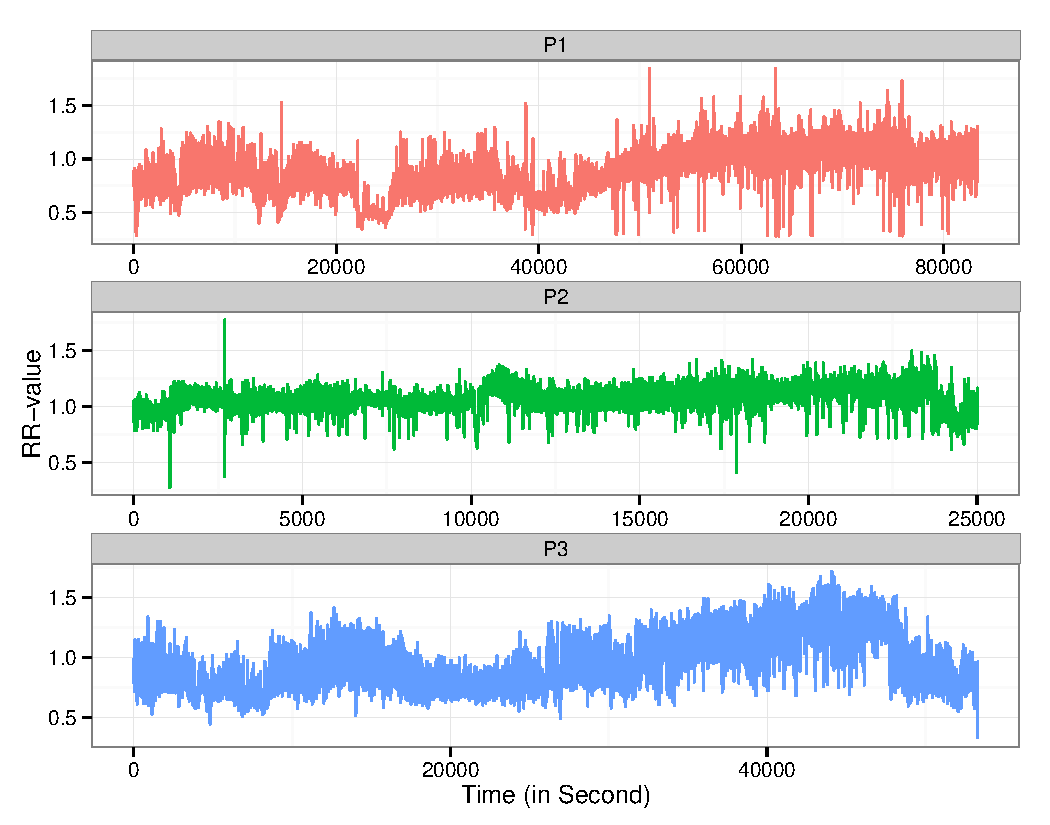
\includegraphics[width=\maxwidth]{figure/longSeriesPlot-1} \caption[Long Term (< 12 hours) rr-measurement for 3 differnt persons]{Long Term (< 12 hours) rr-measurement for 3 differnt persons}\label{fig:longSeriesPlot}
\end{figure}


\end{knitrout}


Long term (> 12 hours) measurements were also collected to explore the 24 hour rhythm and to detect the sleep and awake periods. It is expected to seet he difference between different activities such as resting (including sleeping) and active periods from the collected samples. Figure-\ref{fig:longSeries} shows such long-term series for 3 different persons.

In the similar manner, short term measurements of different types of activity such as running, walking, cycling and sleeping were also collected for making a classification/ prediction (fig-\ref{fig:st.rrPlot}). The blood sugar measurements together with long term measurements of HRV is collected. The heart rate is changing when different hormones are released. The expected correlation between HRV and glucose is difficult to find because there are so many other factors that also influences the HRV. Both the glucose series and the HRV series were transformed to the frequency domain by short time Fourier analysis, and the series were analyzed by PCA and PLSR to see if we could find the expected correlation.

\begin{knitrout}
\definecolor{shadecolor}{rgb}{0.969, 0.969, 0.969}\color{fgcolor}\begin{figure}[H]
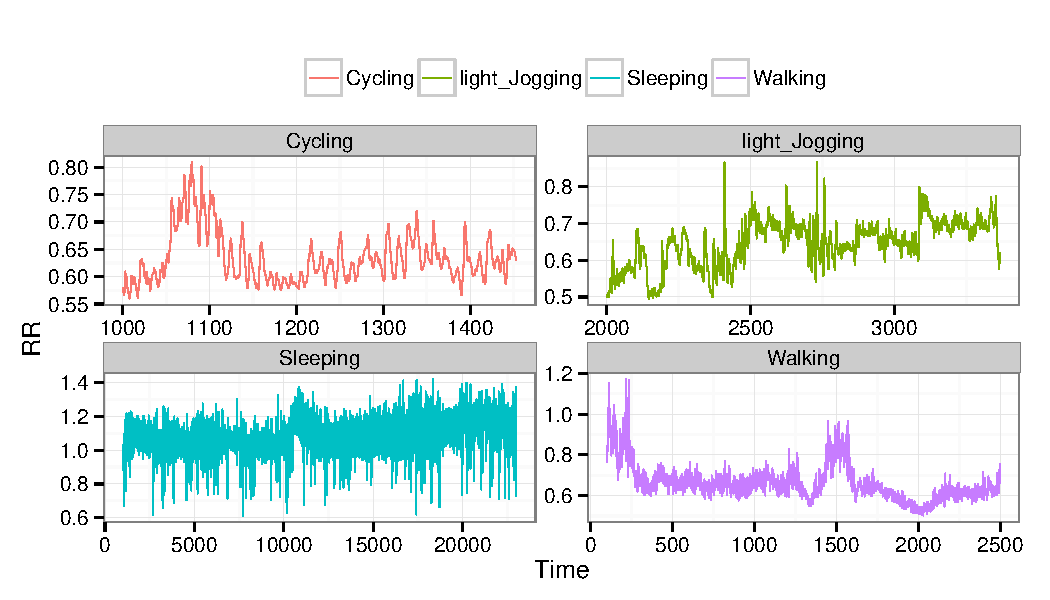
\includegraphics[width=\maxwidth]{figure/st_rrPlot-1} \caption[Short term RR-series for different activities]{Short term RR-series for different activities}\label{fig:st.rrPlot}
\end{figure}


\end{knitrout}
\section{Noise Handling}
Very short intervals are filtered by the device while very long intervals must be handled by the software. On one hand, if artefacts are not removed, the reported ratio between high and low frequencies will be too high, the reported body resilience can be too pessimistic. (A ratio above 2 indicates a low body resilience.) On the other hand, when artefacts are removed, we also remove important information about health issues, and the reported body resilience can be too optimistic.

Filtering of the signal is a tradeoff between interpreting noise and removing information. In sport applications, the analysis are usually run on filtered signals. In medicine, the analysis are often performed both on the filtered and the unfiltered signal.

\section{Artefact filtering}
Filtered with unfiltered series were compared with the Kubios HRV open software. For short term measurements, the artefacts had a large impact on the values in the time domain. In the frequency domain, more low frequency components were present in the unfiltered series, for both short time and long term measurements. Those low frequency components were not masking the frequencies we were looking for, and therefore the analysis in the frequency domain were run on unfiltered series. We only had to be aware of the situation such as,
\begin{itemize}
\item The low frequencies could mean either a noisy signal or the presence of a health issue.
\item The LF/HF ratio can therefore not be interpreted in an unfiltered signal. 
{\color{red}\texttt{Right: comparing a filtered and unfiltered long term measurement in time domain and frequency domain.}}
\end{itemize}

\section{Signal resampling}
The RR series were resampled to get the data points evenly spaced in time (method: linear and spline interpolation). The highest speed for the heart rate in an adult is 240 bpm, or 240/60 bps which is 4 Hz (RR interval=0.25 sec). The sampling rate has then to be 2*4= 8 Hz to detect such high frequencies. A normal heart rate is not above 120 bpm, or 120/60 bps which is 2 Hz (RR interval=0.5 sec). A sampling rate of 2*2=4 Hz is therefore considered to be good enough for practical use. We have used the sampling rate 4 Hz for preprocessing in R and 8 Hz for preprocessing in Matlab (calculation on longer series and high sampling rate take longer time).

\chapter{Methods and Results}
Principal Component Analsysis is adopted to foresee the existing pattern in the series before going for the classification of the event. PCA shows that more than 85 percent variation in the dataset is captured by just three principal components (fig-\ref{fig:pca.plot}). Since principal components are the linear combinations of all the variables with selected coefficients such that the combination carries most of the variations in its first few components.

\begin{knitrout}
\definecolor{shadecolor}{rgb}{0.969, 0.969, 0.969}\color{fgcolor}\begin{figure}[H]
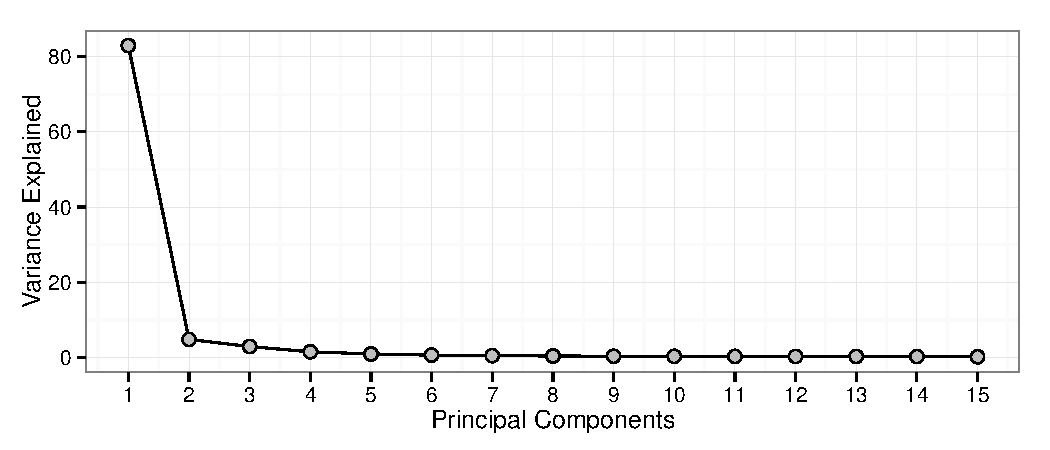
\includegraphics[width=\maxwidth]{figure/pca_plot-1} \caption[Variance explained in Principal Component Analysis]{Variance explained in Principal Component Analysis}\label{fig:pca.plot}
\end{figure}


\end{knitrout}

The first principal componets is plotted against second principal component in figure - \ref{fig:pca.score.plot}. When the scores are colored according to the events they belong, A clear seperation between the active periods and sleeping(relaxing) state is visiable. The figure shows that the first principal component is responsible for most of the separation between active and passive activities.

\begin{knitrout}
\definecolor{shadecolor}{rgb}{0.969, 0.969, 0.969}\color{fgcolor}\begin{figure}[H]
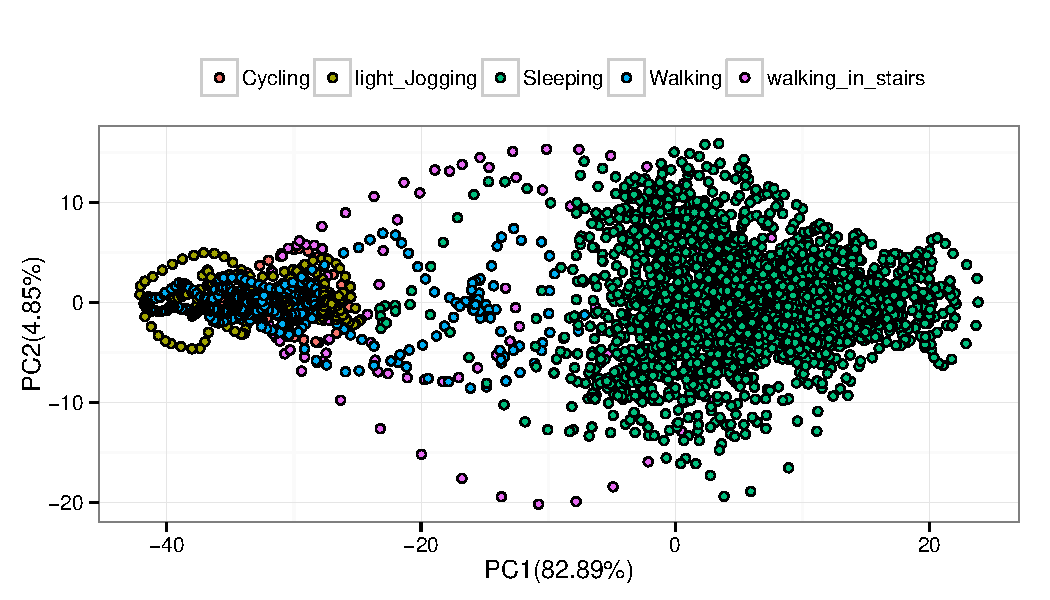
\includegraphics[width=\maxwidth]{figure/pca_score_plot-1} \caption[Score plot for Principal component analysis colored with various activities]{Score plot for Principal component analysis colored with various activities}\label{fig:pca.score.plot}
\end{figure}


\end{knitrout}

\chapter{Discussions and Conclusions}


\nocite{R-data.table,R-ggplot2,R-knitr,R-pls,R-plyr,R-readr,R-reshape2}
\printbibliography

\begin{appendices}
\chapter{Relevant Plots}
\section{Noise Handling}
\begin{figure}[H]
\centering
\begin{subfigure}[t]{\textwidth}
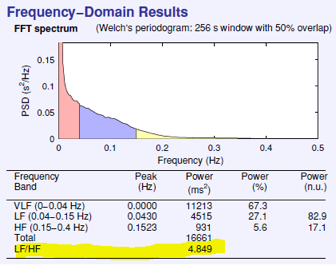
\includegraphics[width = 0.2\textwidth]{figure/noiseHandling/NoiseHandling-1}
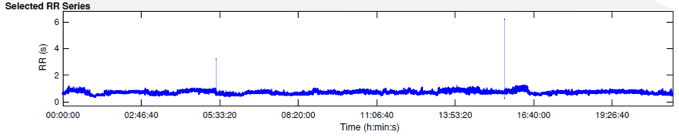
\includegraphics[width = 0.8\textwidth]{figure/noiseHandling/NoiseHandling-5}
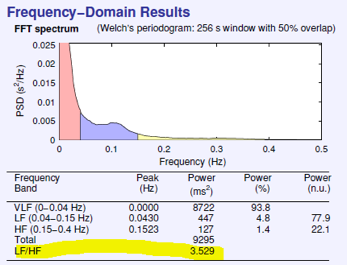
\includegraphics[width = 0.2\textwidth]{figure/noiseHandling/NoiseHandling-2}
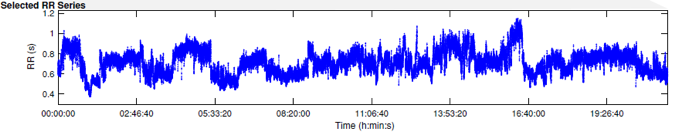
\includegraphics[width = 0.8\textwidth]{figure/noiseHandling/NoiseHandling-6}
\caption{Sample-1: The peaks are most likely noise. Analysis on the unfiltered signal gives too pessimistic LF/HR ratio.}
\label{fig:noiseHandling-s1}
\end{subfigure}
\begin{subfigure}[t]{\textwidth}
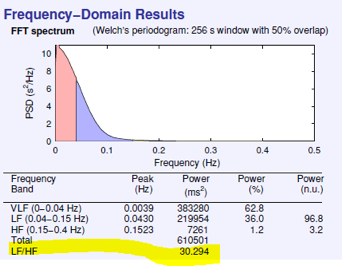
\includegraphics[width = 0.2\textwidth]{figure/noiseHandling/NoiseHandling-3}
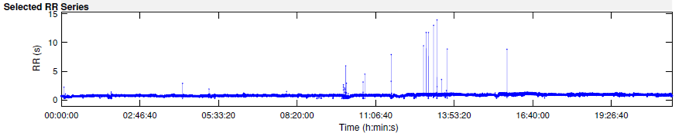
\includegraphics[width = 0.8\textwidth]{figure/noiseHandling/NoiseHandling-7}
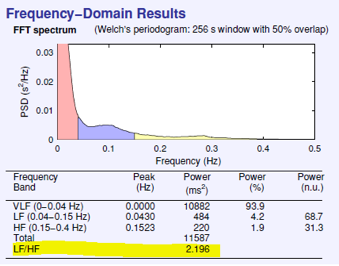
\includegraphics[width = 0.2\textwidth]{figure/noiseHandling/NoiseHandling-4}
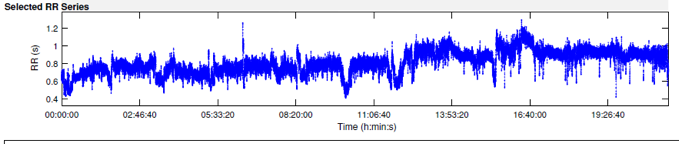
\includegraphics[width = 0.8\textwidth]{figure/noiseHandling/NoiseHandling-8}
\caption{Sample-2: The peaks are reflecting a health issue. Analysis on the filtered signal gives too optimistic LF/HR ratio}
\label{fig:noiseHandling-s2}
\end{subfigure}
\caption{Example of various cases of noise and information included in a RR-series}
\label{fig:noiseHandling}
\end{figure}
\end{appendices}

\end{document}
